\chapter{Approach}\label{ch:approach}

In this research's scope, we propose a new concurrent range-locking design.
We developed our concurrent range lock based on the \texttt{LockFreeSkipList} proposed by Herlihy et al.~\parencite{herlihy2020art}.
In summary, our concurrent range lock uses atomic operations (\texttt{compareAndSet()}) to manage \texttt{Node} references without locks, which enhances performance in multithreaded environments.
When adding a \texttt{Node}, the process starts at the lowest level and moves upward to ensure immediate visibility.
Removing a \texttt{Node} involves marking nodes from the top down before unlinking them.
Furthermore, it relaxes strict structural maintenance of higher levels, focusing on the bottom-level list for set representation, which offers improved scalability and efficiency.

\section{Skip List}\label{sec:skip-list}

A skip list is a probabilistic data structure.
It allows fast search, insertion, and deletion.
It is an alternative to balanced trees, such as AVL trees or red-black trees~\parencite{pugh1990skip, pugh1990skip2}.
The key idea of a skip list is to use multiple layers of sorted linked lists to maintain elements, where each layer is an \("\)express lane\("\) for faster traversal.

\begin{figure}[h]
    \centering
    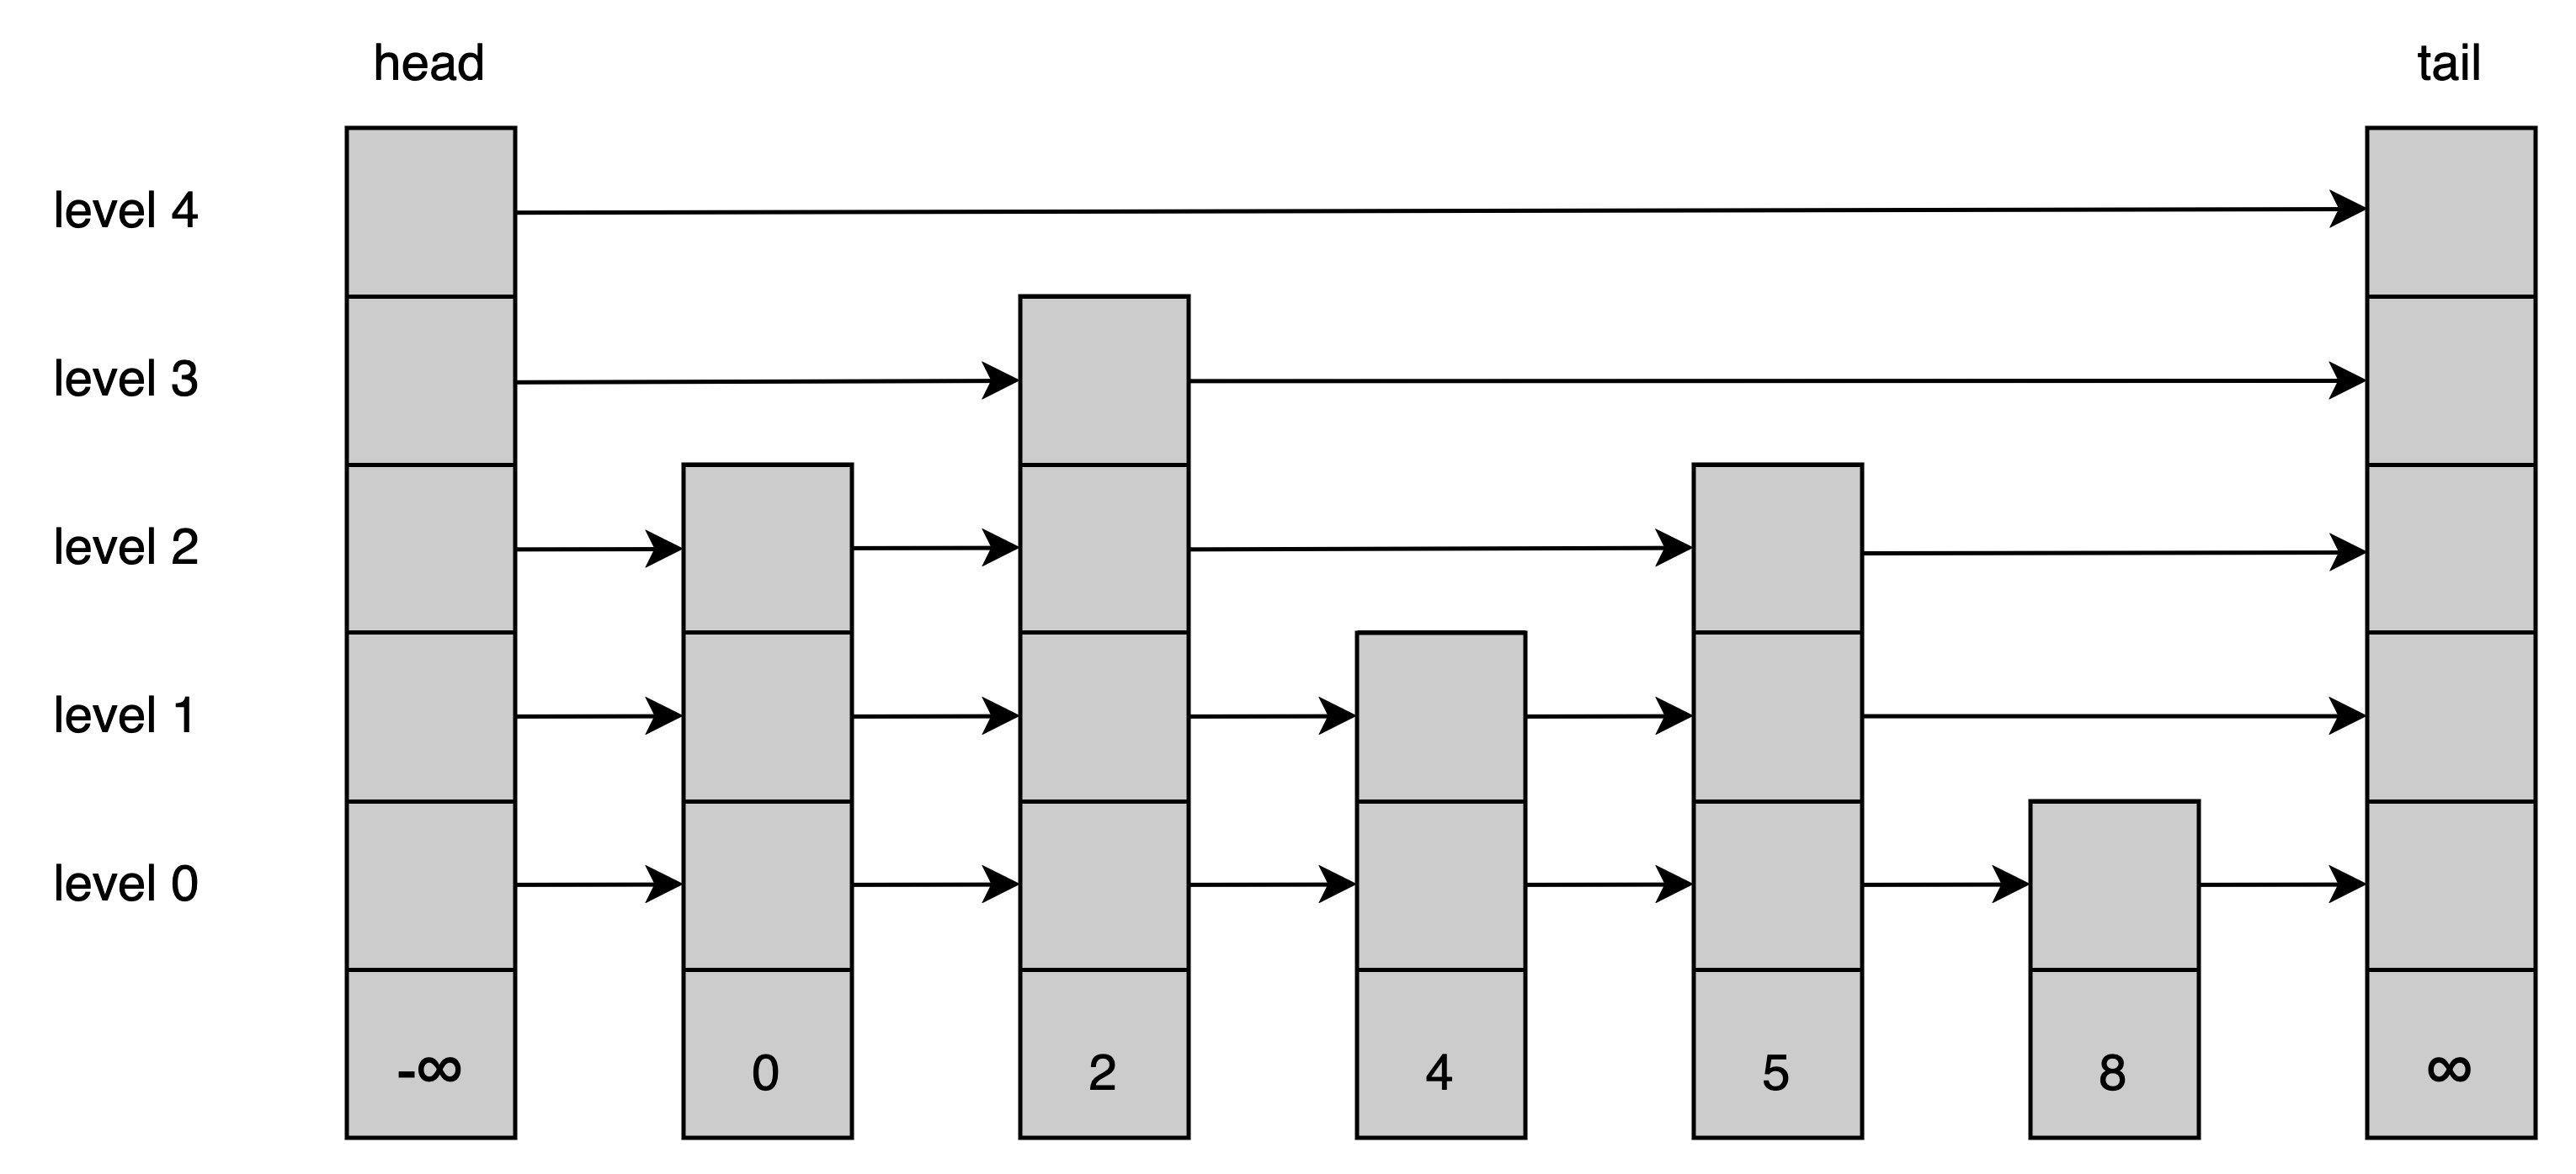
\includegraphics[width=0.8\textwidth]{./figures/skiplist.png}
    \caption{Skip List: In this example, it has five levels of sorted linked lists. \\
 Each \texttt{Node} has an unique key.}
    \label{fig:skiplist}
\end{figure}

\subsection*{How it work}\label{subsec:howitwork}

\textbf{Multiple Layers:} A skip list consists of multiple layers where the bottom-most layer is a regular sorted linked-list.
Each higher layer acts as an \("\)express lane\("\) that speeds up access by skipping over multiple elements from the layer below.
Nodes in higher layers provide shortcuts, allowing faster traversal across the list and effectively reducing the time complexity of search operations.

\textbf{Probabilistic Balancing:} Each \texttt{Node} is created with a random top level and belongs to all lists up to that level.
Top levels are chosen so that the expected number of nodes in each level's list decreases exponentially.
Let \(0 < p < 1\) be the conditional probability that a \texttt{Node} at level \(i\) also appears at level \(i + 1\).
All nodes appear at level \(0\).
The probability that a \texttt{Node} at level 0 also appears at level \(i > 0\) is \( p^i\).
For example, with \(p = 1/2\), \(1/2\) of the nodes are expected to appear at level \(1\), \(1/4\) at level 2, and so on, providing a balancing property like the classical sequential tree-based search structures, except without the need for complex global restructuring.
This random generation ensures that the list structure remains balanced.
Consequently, skip list insertion and deletion algorithms are much simpler and faster than equivalent algorithms for balanced trees.

\begin{figure}[hbt!]
    \centering
    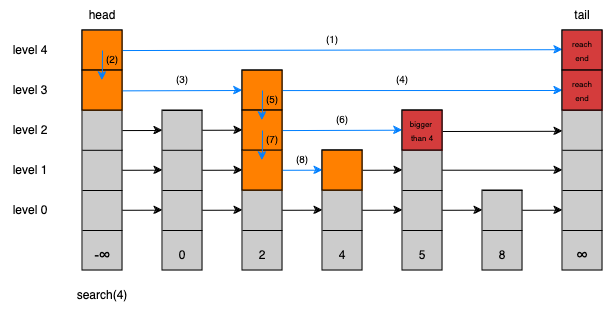
\includegraphics[width=0.8\textwidth]{./figures/skiplistsearch.png}
    \caption{Skip List: In this example, the list searches for a \texttt{Node} with value 4. It starts on the head \texttt{Node} on the highest level, tries to move horizontally until it reaches a greater value than 4, and then goes down a level and repeats. The number noted on the arrows implies the order of the traversal.}
    \label{fig:skiplistsearch}
\end{figure}

\textbf{Search Operation:} To search for an element, the algorithm starts at the topmost layer and moves horizontally through the elements of that layer.
When it encounters an element greater than the target, it drops to the next lower layer and continues the search horizontally.
This process of horizontal traversal and vertical descent continues until the target element is found or the search reaches the bottom-most layer without finding the target.
The hierarchical structure allows for logarithmic search time.

\textbf{Insertion and Deletion:} Inserting an element involves locating the appropriate position in the bottom-most layer, placing the element there, and then potentially promoting the element to higher layers.
Each promotion step is independent, ensuring the probabilistic balancing of the structure.
Deleting an element requires removing it from all layers in which it appears, which is straightforward once the element is located using the search algorithm.
The process of updating references in multiple layers ensures that the skip list remains balanced and efficient for subsequent operations.


\subsection*{Skiplist are suitable for concurrent range lock}
Despite their theoretically poor worst-case performance, skip lists rarely exhibit worst-case behavior, making them efficient in most scenarios.
For instance, in a dictionary with over 250 elements, the likelihood of a search taking more than three times the expected duration is less than one in a million~\parencite{pugh1990skip2}.

Skip lists are, therefore, ideal for implementing range locks, offering a balanced structure that improves concurrency.

% Duy: compare this with Linked-list. If possible, compare this with Bitmap or ......
\begin{table}[h!]
    \centering
    \begin{tabular}{|c|c|c|c|}
        \hline
        \textbf{Operation} & \textbf{Best Case} & \textbf{Average Case} & \textbf{Worst Case} \\ \hline
 Search, Insert, Delete & $O(1)$ & $O(\log n)$ & $O(n)$ \\ \hline
    \end{tabular}
    \caption{Time complexities of skip list operations}
    \label{tab:skiplisttimecomplexity}
\end{table}

\clearpage

\section{Concurrent Range Lock}\label{sec:concurrent-range-lock}

In this section, we will focus on the algorithm of concurrent range lock in details. For the sake of simplicity, we use \texttt{uint64\_t} for our pseudocode provided in this section. In our open-source C++ implementation, we use the template to enable generic
programming. For furthur detail, please checkout our \href{https://github.com/thuaduc/concurrent-range-locking}{ open-source code}.

\subsection{Concurrent Range Lock API}\label{subsec:api}

The \texttt{ConcurrentRangeLock} class provides a concurrent mechanism to manage range-based locks.
Its primary API includes methods for locking and unlocking ranges.
Each range is stored in a single \texttt{Node}.

The \texttt{tryLock} method attempts to acquire a lock for the specified range \texttt{[start, end]}, returning \texttt{true} on success and \texttt{false} otherwise.
The \texttt{releaseLock} method releases the lock for the range \texttt{[start, end]}, with \texttt{true} indicating success and \texttt{false} if the range was not found or an error occurred.
We will discuss these methods in subsection \ref{subsec:tryLock} and \ref{subsec:releaseLock}.

The two primary methods rely heavily on \texttt{find} methods such as \texttt{findInsert}, \texttt{findExact}, and \texttt{findDelete}, which handle insertion finding, exact range finding, and physical deletion of ranges, respectively. We will discuss these methods in section \ref{subsec:find}.

\begin{figure}[h]
    \centering
    \lstinputlisting[style=mystyle,caption={Pseudocode for ConcurrentRangeLock API},label={lst:api}]{code/api.txt}
\end{figure}

\clearpage

\subsection{Node}\label{subsec:node}

\texttt{Node} is the base of our \texttt{ConcurrentRangeLock} structure.
Each \texttt{Node} contains \textbf{\texttt{start}} and \textbf{\texttt{end}}, which represents range.
\texttt{Node} also uses an array of \textbf{\texttt{AtomicMarkableReference}} (more details in section \ref{subsec:atomicmarkablereference}) to maintain forward links at each level, which allows for efficient traversal and updates.
\texttt{Node} provides the following methods:

\begin{itemize}
    \item \texttt{initialize}: sets up a \texttt{Node} with specific range and level values.
    \item \textbf{\texttt{initializeHead}}: configures the head \texttt{Node} with forward pointers directed to a provided tail \texttt{Node}, establishing the initial structure.
    \item \texttt{getTopLevel()}, \texttt{getStart()}, \texttt{getEnd()}: accessor methods to retrieve the Node's properties.
\end{itemize}

\begin{figure}[h]
    \centering
    \lstinputlisting[style=mystyle,caption={Pseudocode for Node structure},label={lst:node}]{code/node.txt}
\end{figure}

\clearpage

\subsection{AtomicMarkableReference} \label{subsec:atomicmarkablereference}

The \texttt{AtomicMarkableReference} class uses a single atomic variable, \texttt{atomicRefMark}, to store a packed representation of both the reference (specifically, a \texttt{Node}) and a mark. If the mark is \texttt{1}, it indicates that the \texttt{Node} it references is softly deleted. These values are packed and unpacked using bitwise operations, where the least significant bit represents the mark.

Listing \ref{lst:atomicmarkablereference} provides the pseudo code for \texttt{AtomicMarkableReference}.

The \texttt{pack} method combines a \texttt{Node} pointer and a boolean mark into a single \texttt{uintptr\_t} value by encoding the pointer into the lower bits and the mark into the highest bit. Conversely, the \texttt{unpack} method decodes this packed value to retrieve the original \texttt{Node} pointer and boolean mark.

To atomically set a new \texttt{Node} pointer and mark value, the \texttt{store} method uses relaxed memory ordering.

The \texttt{compareAndSet} method performs an atomic update of both the reference and mark if they match the expected values, employing acquire-release memory ordering for proper synchronization.

The \texttt{attemptMark} method focuses on updating the mark alone, provided that the current reference matches the expected one and the mark differs. If the update succeeds, it returns \texttt{true}; otherwise, it returns \texttt{false}.

To retrieve the current reference and mark, the \texttt{get} method is used, which stores the mark in a provided boolean pointer. In contrast, the \texttt{getReference} method simply returns the current reference without accessing the mark.

\begin{figure}[!p]
    \centering
    \lstinputlisting[style=mystyle,caption={AtomicMarkableReference},label={lst:atomicmarkablereference}]{code/atomicmarkablereference.txt}
\end{figure}

\clearpage

\subsection{Find}\label{subsec:find}

Both \texttt{tryLock} and \texttt{releaseLock} methods rely heavily on \texttt{find} methods.
There are several find methods in our implementation that serve different purposes:

\begin{itemize}
    \item \texttt{bool findInsert(uint64\_t start, uint64\_t end, Node** preds, Node** succs)}: checks if the target range \texttt{[start, end]} is free to be inserted.

    \item \texttt{bool findExact(uint64\_t start, uint64\_t end, Node** preds, Node** succs)}: checks if the target range \texttt{[start, end]} is already present in the skip list.

    \item \texttt{void findDelete(uint64\_t start, uint64\_t end)}: finds the target range \texttt{[start, end]} from the skip list to physically delete the Node which contains the corresponding range.
\end{itemize}

These \texttt{findInsert} and \texttt{findExact} methods also fill in the \texttt{preds[]} and \texttt{succs[]} arrays with the target node's ostensible predecessors and successors at each level.
Because the goal of \texttt{findDelete} is only to snip out all the deleted Node, there is no need to fill any array.

Nevertheless, these methods have to maintain the following two properties:

\begin{itemize}
    \item During traversal, they need to skip over marked nodes.
    They use \texttt{compareAndSet()} (as discussed in \ref{subsec:atomicmarkablereference}) to ensure that remove all softly deleted Node on the way.
    \item Every \texttt{preds[]} reference is to a node with a key strictly less than the target.
\end{itemize}

\vspace{15pt}

\begin{figure}[!p]
    \centering
    \lstinputlisting[style=mystyle,caption={General pseudocode for find methods},label={lst:find}]{code/find.txt}
\end{figure}

\subsubsection{Algorithm in details}
The \texttt{find()} method starts by traversing the LockFreeSkipList from the \texttt{topLevel} of the head sentinel, which has the maximal allowed node level.
It proceeds down the list level by level, filling in the \texttt{preds} and \texttt{succs} nodes.
These nodes are repeatedly advanced until \texttt{pred} refers to a node with the largest value on that level that is strictly less than the target key (lines 13--29).

While traversing, it repeatedly snips out marked nodes from the current level as they are encountered (lines 15--22) using a \texttt{compareAndSet()}.
The \texttt{compareAndSet()} function validates that the following field of the predecessor still references the current Node.

Once an unmarked \texttt{curr} node is found (line 23), it is tested to see if its \texttt{start} is greater than or equal to the target \texttt{start}.
If so, \texttt{pred} is advanced to \texttt{curr}, \texttt{curr} is advanced to \texttt{succ}, and the traverse continues.
Otherwise, the current range of \texttt{pred} is the immediate predecessor of the target node.
The \texttt{find()} method then breaks out of the current level search loop, saving the current values of \texttt{pred} and \texttt{curr} (line 26--32).

The \texttt{find()} method continues this process until it reaches the bottom level.
An important point is that each level's traversal maintains the previously described properties.
Specifically, if a node with the target key is in the list, it will be found at the bottom level even if nodes are removed at higher levels.
When traversal stops, \texttt{pred} refers to a predecessor of the target node.
The method descends to each next lower level without skipping over the target node.
If the Node is in the list, it will be found at the bottom level.
Additionally, if the Node is found, it cannot be marked because if it were marked, it would have been snipped out in lines 15--22.
Thus, the condition test on line 35 only needs to check if there are overlap ranges (\texttt{findInsert}) or if the start and end of the Node match the target start and end (\texttt{findExact}).
\begin{enumerate}
    \item \texttt{findInsert}:
    \begin{lstlisting}[style=nonum, label={}]
    return (!(start > pred->getEnd() && end < curr->getStart()));
    \end{lstlisting}
    \item \texttt{findExact}:
    \begin{lstlisting}[style=nonum, label={}]
    return (start == curr->getStart() && end == curr->getEnd());
    \end{lstlisting}
\end{enumerate}

The linearization points for both successful and unsuccessful calls to the \texttt{find()} method occur when the \texttt{curr} reference at the bottom-level list is set, either at line 11 or line 20, for the last time before the success or failure of the \texttt{find()} call is determined at line 35.

\clearpage

\subsection{Try Lock}\label{subsec:tryLock}

The \texttt{tryLock} method, shown in Listing \ref{lst:tryLock}, utilizes \texttt{findInsert()} to check if a node with the range \texttt{[start, end]} already exists. If found, \texttt{tryLock} returns \texttt{false}, otherwise, it creates a new node and attempts to insert it into the list. The node is inserted starting from the bottom level, with \texttt{compareAndSet()} ensuring the integrity of the insertion. If any insertion fails due to concurrent changes, \texttt{findInsert()} is called again to update the predecessors and successors, and the process repeats until successful.

\vspace{15pt}


\begin{figure}[!p]
    \centering
    \lstinputlisting[style=mystyle,caption={Pseudocode for tryLock method},label={lst:tryLock}]{code/trylock.txt}
\end{figure}

\subsubsection*{Algorithm in details}
The \texttt{tryLock} method, shown in listing \ref{lst:tryLock}, uses \texttt{findInsert()}, show in listing \ref{lst:find}, to determine whether a node with range \texttt{[start, end]} is already in the list (line 7). \texttt{tryLock} also calls \texttt{findInsert()} to initialize the preds[] and succs[] arrays to hold the new node's ostensible predecessors and successors.
If an unmarked node with the target key is found in the bottom-level list, \texttt{findInsert()} returns \texttt{accurate} and the \texttt{tryLock} method returns \texttt{false}, indicating that the key is already in the set. The unsuccessful \texttt{tryLock}'s linearization point is the same as the successful \texttt{findInsert()}'s (line 8). If no node is found, the next step is to add a new node with the key into the structure.

A new node is created with a randomly chosen top-level (lines 10--11). The node's next references are unmarked and set to the successors returned by the \texttt{findInsert()} method (lines 13--15).
The next step is to try to add the new node by linking it into the bottom-level list between the \texttt{preds[0]} and \texttt{succs[0]} nodes returned by \texttt{findInsert()}. We use the \texttt{compareAndSet()} method to set the reference while validating that these nodes still refer one to the other and have not been removed from the list (line 17). If the  \texttt{compareAndSet()} fails, something has changed and the call restarts. If the  \texttt{compareAndSet()} succeeds, the item is added, and line 17 is the call's linearization point.
The {findInsert()} then links the node in at higher levels (lines 21--25). For each level, it attempts to splice the node by setting the predecessor, if it refers to the valid successor, to the new node (lines 22--23). If successful, it breaks and moves on to the next level. If unsuccessful, then the node referenced by the predecessor must have changed, and \texttt{findInsert()} is called again to find a new valid set of predecessors and successors (line 24). We discard the result of calling \texttt{findInsert()} because we care only about recomputing the ostensible predecessors and successors on the remaining unlinked levels. Once all levels are linked, the method returns true (line 27).
The \texttt{releaseLock} method, shown in listing \ref{lst:releaseLock}, calls \texttt{findExact()} to determine whether an unmarked node with a matching range \texttt{[start, end]} is in the bottom-level list (line 7). If no node is found in the bottom-level list, or the node with a matching range \texttt{[start, end]} is marked, the method returns false. The linearization point of the unsuccessful \texttt{releaseLock} is that of the \texttt{findExact()} method called in line 7.

If an unmarked node is found, the method logically removes the associated key from the abstract set and prepares it for physical removal. This step uses the set of ostensible predecessors (stored by \texttt{findExact()} in \texttt{preds[]}) and the victim (returned from \texttt{findExact()} in \texttt{succs[]}). First, starting from the top-level, all links up to and \textbf{not including} the bottom-level link are marked (Lines 12--20) by repeatedly reading next and its mark and applying \texttt{attemptMark()}. If the link is found to be marked (either because it was already marked or because the attempt succeeded), the method moves on to the next-level link. Otherwise, the current level's link is reread since another concurrent thread must have changed it, so the marking attempt must be repeated.

Once all levels but the bottom one have been marked, the method marks the bottom-level's next reference. If successful, this marking (line 27) is the linearization point of a successful \texttt{releaseLock}. The \texttt{releaseLock} method tries to mark the next field using \texttt{compareAndSet()}. If successful, it can determine that it was the thread that changed the mark from false to true. Before returning true, the \texttt{findDelete()} method is called. This call is an optimization: \texttt{findDelete()} physically removes all links to the node it is searching for.

On the other hand, if the  \texttt{compareAndSet()} call fails, but the next reference is marked, then another thread must have concurrently removed it, so \texttt{releaseLock} returns false. The linearization point of this unsuccessful \texttt{releaseLock} is the linearization point of the \texttt{releaseLock} method by the thread that successfully marked the next field. Notice that this linearization point must occur during the \texttt{releaseLock} call because the \texttt{findExact()} call found the node unmarked before it found it marked.

Finally, if the \texttt{compareAndSet()} fails and the node is unmarked, the next node must have changed concurrently. Since the victim is known, there is no need to call find() again, and \texttt{releaseLock} simply uses the new value read from next to retry the marking.

\clearpage

\subsection{Release Lock}\label{subsec:releaseLock}

The \texttt{releaseLock} method first calls \texttt{findExact()} to locate an unmarked node with the specified range \texttt{[start, end]}. If found, it marks all levels of the node except the bottom one, preparing the node for removal. The method then attempts to mark the bottom-level link using \texttt{compareAndSet()}, which serves as the linearization point for a successful \texttt{releaseLock}. If marking fails due to concurrent modifications, the method retries or returns false, depending on the state of the node.

\vspace{15pt}

\begin{figure}[!p]
    \centering
    \lstinputlisting[style=mystyle,caption={Pseudocode for releaseLock method},label={lst:releaseLock}]{code/releaselock.txt}
\end{figure}

\subsubsection*{Algorithm in details}

The \texttt{releaseLock} method, shown in listing \ref{lst:releaseLock}, calls \texttt{findExact()} to determine whether an unmarked node with a matching range \texttt{[start, end]} is in the bottom-level list (line 7).
If no node is found in the bottom-level list, or the node with a matching range \texttt{[start, end]} is marked, the method returns false.
The linearization point of the unsuccessful \texttt{releaseLock} is that of the \texttt{findExact()} method called in line 7.

If an unmarked node is found, the method logically removes the associated key from the abstract set and prepares it for physical removal.
This step uses the set of ostensible predecessors (stored by \texttt{findExact()} in \texttt{preds[]}) and the victim (returned from \texttt{findExact()} in \texttt{succs[]}).
First, starting from the top-level, all links up to and \textbf{not including} the bottom-level link are marked (Lines 12--20) by repeatedly reading next and its mark and applying \texttt{attemptMark()}.
If the link is found to be marked (either because it was already marked or because the attempt succeeded), the method moves on to the next-level link.
Otherwise, the current level's link is reread since another concurrent thread must have changed it, so the marking attempt must be repeated.

Once all levels but the bottom one have been marked, the method marks the bottom-level's next reference.
If successful, this marking (line 27) is the linearization point of a successful \texttt{releaseLock}. The \texttt{releaseLock} method tries to mark the next field using \texttt{compareAndSet()}.
If successful, it can determine that it was the thread that changed the mark from false to true. Before returning true, the \texttt{findDelete()} method is called. This call is an optimization: \texttt{findDelete()} physically removes all links to the node it is searching for.

On the other hand, if the  \texttt{compareAndSet()} call fails, but the next reference is marked, then another thread must have concurrently removed it, so \texttt{releaseLock} returns false.
The linearization point of this unsuccessful \texttt{releaseLock} is the linearization point of the \texttt{releaseLock} method by the thread that successfully marked the next field.
Notice that this linearization point must occur during the \texttt{releaseLock} call because the \texttt{findExact()} call found the node unmarked before it found it marked.

Finally, if the \texttt{compareAndSet()} fails and the node is unmarked, the next node must have changed concurrently.
Since the victim is known, there is no need to call find() again, and \texttt{releaseLock} simply uses the new value read from next to retry the marking.

% Duy: Lifecycle viết phức tạp và khó theo dõi quá. Một cách viết khác là kiểu như draw 1 cái state machine như trong paper của anh, Figure 4.
% Duy: Sau đó tại mỗi step thì viết thành 1 subsection, APIs liên quan hay internal state gì đó. Kết cái subsection dó thành expected state rồi transition sang subsection tiếp theo.
% Duy: 1 ví dụ high-level lifecycle through the whole story: https://www.vldb.org/pvldb/vol16/p1426-alhomssi.pdf -- Figure 2
% Duy: Để ý cái section 3.5 -- Putting Everything Together, có thể làm thêm 1 cái như này nữa cũng ổn
